\subsection{Experimental setup}\label{subsec:setup}

We fine-tune LoRA adapters of rank $r = 16$ on four base models,
Llama-3.1-8B-Instruct, Mistral-7B-v0.3, Qwen2.5-7B-Instruct and Yi-1.5-9B-Chat,
for four unrelated tasks: grade-school mathematics (GSM8K), instruction
following (Alpaca), code generation (Magicoder) and English-to-German
translation (WMT19). Each base has two kinds of cohort. In a \emph{shared}
cohort all four task configurations carry one global seed, so all four
adapters are created from the same random state; we train three such cohorts
with seeds 1, 2 and 3. In an \emph{independent} cohort each task has its own
seed; we train three of these as well. The seed enters training in three
places: the random state when the adapter is created, the order of the data
and the dropout masks, and the split of the data. The two arms differ in all
three, and \S\ref{subsec:seeds} separates them.

Three of the four adapters improve on the base model by $10$ to $70\%$ on their
own task. The translation adapter did not learn its task: a data-loading defect
trained it on
an unshuffled, single-domain prefix of its corpus, and on every base and in
both arms it is beaten at translation by the base model or by another adapter. Both arms
contain the same weak member, so every comparison in this paper, which is
always between the two arms, is matched. Cohorts retrained with the fix on two
bases reproduce every result below.

Merged models are scored in two units: the worst-task excess negative
log-likelihood (the largest, over tasks, of the merged model's NLL on a task
minus that of the task's own adapter), and downstream accuracy, exact match on
$500$ GSM8K problems and pass@1 on the $164$ HumanEval problems. Every merge is
truncated back to rank $r$, as for deployment; \S\ref{sec:merging} reports
what changes without truncation. Initial versions of the code for some
parts of the experiments and analyses were produced with an AI coding
assistant, Claude (Anthropic); the authors reviewed and revised the code, which
is public together with the per-cell results it produced
(\S\ref{sec:conclusion}).

\subsection{Why a shared start collapses the subspaces}\label{subsec:why}

The update $BA$ maps inputs through the row space of $A$, so the input
subspace of each update lies inside $V_t$. Because $B = 0$ at
initialisation, the gradient with respect to $A$ is proportional to $B$ and
vanishes at the first step, so $A$ moves comparatively little over training.
We measured how little on a cohort whose initial $A$ was saved before the first
optimiser step: by the end of training $A$ has moved $13\%$ of its own norm.
If every $A_t$ starts from the same matrix and each moves $13\%$, the $T$ task
subspaces stay close to the starting one and therefore to each other, whatever
the tasks.

The same measurement separates the start from the training
(Figure~\ref{fig:collapse}a). A shared cohort and an independent cohort drift
by $0.1308$ and $0.1303$ of their initial norm, a difference of $0.0005$, and
end at median principal cosines of $0.996$ and $0.047$. Training moves $A$ by the same amount in both, so the collapse is set
by where the adapters started and not by anything training does.

\subsection{The initialisation seed alone decides}\label{subsec:seeds}

\begin{table}[pos=tbp]
\centering
\small
\caption{The seed ablation on Llama-3.1-8B. The initialisation seed sets the
random state when the adapters are created; the trainer seed sets the data
order and dropout. ``Shared'' means one seed for all four tasks, ``own'' one
per task. The data split is the same in all four cohorts. Excess is the
worst-task NLL excess of adapter-only RegMean at $\lambda = 10^{-6}$ and of
task arithmetic.}
\label{tab:seeds}
\begin{tabular}{llcccc}
\toprule
init seed & trainer seed & median cosine & $\kappa(\bar H)$
 & RegMean excess & task arithmetic excess \\
\midrule
shared & shared & 0.995 & $1.11\times10^{4}$ & 0.342 & 0.216 \\
shared & own    & 0.995 & $1.07\times10^{4}$ & 0.368 & 0.214 \\
own    & shared & 0.047 & 1.55 & 0.065 & 0.218 \\
own    & own    & 0.047 & 1.55 & 0.071 & 0.221 \\
\bottomrule
\end{tabular}
\end{table}

The argument puts the cause at creation, so the seed in force when the
adapters are created should decide the regime by itself. We tested this with a
registered two-by-two ablation that crosses the initialisation seed with the
trainer seed, holding the data split fixed (Table~\ref{tab:seeds}). The two
cohorts created from one seed are collapsed whether or not they share a
trainer seed, at median cosine $0.995$ and $\kappa(\bar H)$ near $10^{4}$. The
two created from separate seeds are separated whether or not they share one,
at $0.047$ and $1.55$. Adapter-only RegMean follows the initialisation seed:
its excess is $0.34$ to $0.37$ nats on the shared-initialisation cohorts and
$0.07$ on the others. Task arithmetic does not move, at $0.214$ to $0.221$ on
all four. All four registered predictions hold. The data order and dropout,
and with them anything training does differently across tasks, do not decide
the regime; the initial $A$ does.

\subsection{The geometry of the two regimes}\label{subsec:geometry}

\begin{figure}[pos=tbp]
\centering
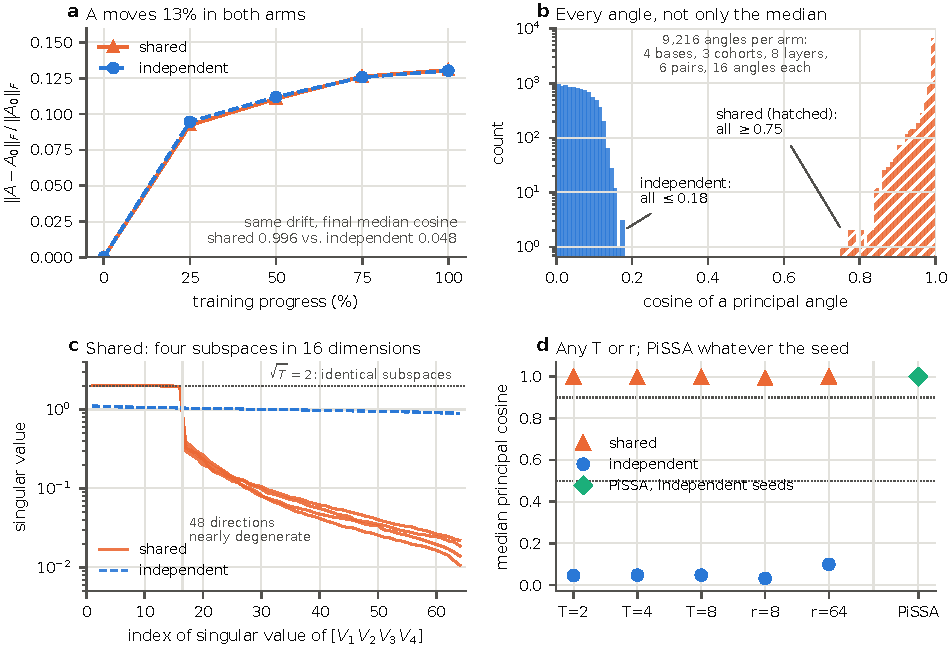
\includegraphics[width=\textwidth]{nc/figures/fig1_collapse.pdf}
\caption{What a shared initialisation does to a cohort. \textbf{(a)} Relative
displacement of $A$ from its initial value during training, on the Llama-3.1-8B
cohorts whose $A_0$ was saved: the two arms move by the same amount.
\textbf{(b)} Every principal cosine between every pair of task subspaces, at
$T = 4$, $r = 16$, pooled over four bases, three cohorts per arm and eight
layers (log count). \textbf{(c)} Singular values of the stacked orthonormal
bases $[V_1\,V_2\,V_3\,V_4]$, median over layers, one line per base: on the
shared arm $16$ values sit at $\sqrt{T} = 2$ and the other $48$ are small.
\textbf{(d)} Median principal cosine on Llama-3.1-8B across task count and
rank, and for a PiSSA cohort trained with four independent seeds. Dotted lines
in (d) mark the audit thresholds of \S\ref{subsec:audit}.}
\label{fig:collapse}
\end{figure}

\begin{table}[pos=tbp]
\centering
\small
\caption{The two regimes at $T = 4$, $r = 16$. The independent arm is the
first of three independent cohorts; the other two agree to three decimals.
Amplification is the norm of the exact interpolator over that of the mean task
update; $T = 4$ is its value for exactly orthogonal subspaces.}
\label{tab:regimes}
\begin{tabular}{lcccccc}
\toprule
 & \multicolumn{2}{c}{median cosine} & \multicolumn{2}{c}{$\kappa(\bar H)$}
 & \multicolumn{2}{c}{amplification} \\
base & shared & indep. & shared & indep. & shared & indep. \\
\midrule
Llama-3.1-8B & 0.995 & 0.047 & $1.76\times10^{4}$ & 1.5 & 48.3 & 4.0 \\
Mistral-7B   & 0.995 & 0.047 & $3.21\times10^{4}$ & 1.5 & 52.3 & 4.0 \\
Qwen2.5-7B   & 0.996 & 0.050 & $2.42\times10^{4}$ & 1.6 & 43.4 & 4.0 \\
Yi-1.5-9B    & 0.997 & 0.047 & $8.30\times10^{4}$ & 1.5 & 64.1 & 4.0 \\
\bottomrule
\end{tabular}
\end{table}

The separation is large and reproducible (Table~\ref{tab:regimes}). On every
base the shared cohort sits at a median principal cosine between $0.995$ and
$0.997$ and the independent cohorts between $0.047$ and $0.050$; the three
independent cohorts agree with each other to three decimals. It holds for every
principal angle, not only the median (Figure~\ref{fig:collapse}b): of the
$9{,}216$ principal cosines on each arm, every shared one is at least $0.75$
and every independent one at most $0.18$. The spectrum of the stacked subspace
bases shows where the dimensions go (Figure~\ref{fig:collapse}c). On the
shared arm, $16$ singular values sit near $\sqrt{T} = 2$ ($1.94$ to $1.96$),
the value for exactly identical subspaces, and the other $48$ fall from $0.3$
to $0.4$ down to $0.01$ to $0.02$, so four rank-$16$ subspaces occupy about
$16$ dimensions. On the independent arm all $64$ lie between $0.88$ and
$1.13$.

The subspaces are near-collinear, not collinear. Four rank-$16$ subspaces in
dimension $d = 4096$ remain linearly independent unless they coincide exactly,
so an exact interpolator exists in both regimes. The regimes differ in how
hard it is to reach. On the shared arm $\kappa(\bar H)$ is $1.8\times10^{4}$
to $8.3\times10^{4}$, against $1.5$ to $1.6$ on the independent arm, and the
exact interpolator is $43$ to $64$ times larger than the mean task update,
against $4.0$. That last value is $T$, the amplification for exactly orthogonal
subspaces, which the independent arm reproduces to within $1.1\%$. The
condition number depends on the curvature model behind $\bar H$, here the
projector model of \S\ref{sec:background}; the principal cosines do not, since
they are properties of the row spaces alone. That is why we lead with them.

\subsection{Task count, rank, training and initialisation scheme}\label{subsec:tr}

The argument above does not depend on $T$ or $r$, so the collapse should hold
at any size, and the conditioning should worsen as more subspaces crowd around
the same start. We tested both on Llama-3.1-8B, training adapters for four
further tasks (Dolly, XSum, CodeAlpaca and English-to-French translation) and
at ranks $8$ and $64$, in both arms. The regime is set by initialisation at
every size (Figure~\ref{fig:collapse}d): shared cohorts sit at median cosine
$0.990$ to $0.999$ and independent ones at $0.032$ to $0.099$. On the shared
arm the conditioning grows with the task count,
$\kappa(\bar H) = 3.9\times10^{3}$, $1.1\times10^{4}$ and $3.9\times10^{4}$ at
$T = 2, 4, 8$, and with the rank, $5.6\times10^{3}$, $1.1\times10^{4}$ and
$4.1\times10^{4}$ at $r = 8, 16, 64$, while on the independent arm the
amplification stays at the orthogonal value $T$ ($1.99$, $4.00$, $7.91$).

No change to training that we tried leaves the regime. We registered seven changes to
training on a shared-initialisation cohort of Llama-3.1-8B, each chosen to move
$A$ further or less far: the learning rate divided or multiplied by $3$, one or
four epochs instead of two, $A$'s learning rate multiplied by $4$, LoRA+ at
its recommended ratio of $16$ between the learning rates of $B$ and $A$, and
$A$'s initial value scaled by $0.25$. Every one stays collapsed, at median
cosine $0.956$ to $0.999$, and the independent counterparts of the two changes
expected to move $A$ furthest stay at $0.047$ and $0.048$. \S\ref{sec:theory} uses these
cohorts to test the theory out of sample, and reports one of them, a smaller
initial $A$, that stays collapsed but lowers the damage to a solver.

A shared seed is not the only route into the regime. PiSSA~\citep{meng2024pissa}
initialises $A$ from the principal singular vectors of the base weight, which
do not depend on the seed. Four PiSSA adapters trained with the independent
arm's four seeds form a collapsed cohort, at median cosine $0.999$, and their
trained row spaces remain at principal cosine $0.9996$ to the base weight's
top-$r$ right singular vectors: training does not move them far enough to
leave the starting subspace.

\subsection{Routes into the regime in practice}\label{subsec:routes}

\paragraph{Library defaults.} Whether two runs create the same $A$ is decided
by what the fine-tuning library does before it creates the adapter, which
\S\ref{subsec:libraries} reads from the source of two widely used stacks. We also
measured it. We fine-tuned Llama-3.2-1B-Instruct on GSM8K and on Alpaca with
Unsloth (2026.5.2) and with LLaMA-Factory (0.9.5), each at its default
settings, twice per task in separate processes. Within each library the
initial $A$ is identical across the two tasks and across the two runs (median
principal cosine $1.000$). After $50$ steps the two tasks' adapters remain at
$0.9996$ under Unsloth and $0.9994$ under LLaMA-Factory. A user who fine-tunes
several tasks with either library without changing its seed obtains a
collapsed cohort.

\paragraph{Continued training.} A common way to build several task adapters is
to start each from an adapter that already exists. We initialised four task
adapters from the $A$ and $B$ of one existing adapter (a Dolly instruction
adapter) and trained each with its own seed, so that no seed is shared. The
cohort is collapsed, at median cosine $0.997$ and
$\kappa(\bar H) = 2.9\times10^{4}$, and adapter-only RegMean at
$\lambda = 10^{-6}$ leaves a worst-task excess of $1.49$ nats, against $0.071$
on the independent cohort of the main grid. Derived adapters reach the regime
without any seed in common.

\paragraph{Other parameterisations and a vision model.} Weight-decomposed LoRA
(DoRA) keeps a LoRA-style $A$, and a shared seed collapses it in the same way:
median cosine $0.995$ for a shared cohort and $0.047$ for an independent one
on Llama-3.1-8B. We measured geometry only, since merging DoRA needs a
treatment of its magnitude vector that this pipeline does not have. Rank-stabilised
LoRA draws $A$ from the same distribution and changes only the scaling, so its
collapse at creation is identical by construction. The regime is not specific
to language models either: rank-$16$ adapters on CLIP ViT-B/32, trained on
eight image classification tasks, sit at median cosine $0.96$ in shared
cohorts and $0.11$ in independent ones (\S\ref{subsec:beyond}).
